\documentclass[11pt,openany]{sprawozdanie-agh}

\usepackage[utf8]{inputenc}
\usepackage[polish]{babel}
\usepackage{listings}

\makeatletter

\begin{document}

\przedmiot{Systemy Informatyczne w Medycynie}
\tytul{Wspomaganie detekcji anomalii guzopodobnych piersi na podstawie automatycznej analizy zdjęć mammografu
}
\podtytul{Dokumentacja}
\kierunek{Informatyka}
\autor{Grzegorz Bylina, Agata Paciorek, Piotr Knop}
\data{Kraków,2014}

\stronatytulowa{}

\tableofcontents

\clearpage

\section{Wstęp teoretyczny}
\subsection{Cel aplikacji}
Celem programu jest porównanie dwóch metod detekcji raka piersi, na podstawie zdjęć mammograficznych w odcieniach szarości. Środowisko, wykorzystane do implementacji to program Matlab.

\subsection{Analiza literatury - metody}
\subsubsection{Oparte na extreme learining machines (ELM)}
\paragraph{Wstępne przygotowanie obrazu\\}
Pierwszym krokiem metody opisanej w \cite{Wang2014} jest usunięcie szumu z obrazu. Uzyskuje się to poprzez zastosowanie filtru medianowego na oknie 3 x 3 piksele. Następnie należy uwydatnić szczegóły obrazu, gdyż są one zamazane. Pierwszym krokiem jest transformacja oryginalnego obrazu w taki sposób, aby podzielić przedział szarości na dwie części, a następnie zredukować zakres przedziału tak, aby uwydatnić przedział kontrastu oryginalnego obrazu.

\paragraph{Wykrycie guza\\}
Kolejnym krokiem jest segmentacja krawędzi. W pierwszej kolejności użyty WMM, czyli ,,wavelet transormation of local modulus maxim'', który zwraca nam wszystkie krawędzie, które podejrzane są o należenie do raka, którego staramy się wykryć. Aby wśród nich znaleźć te, które rzeczywiście należą do krawędzi guza, użyto operacji morfologicznych: erozji, a następnie otwarcia. Mając prawdopodobne krawędzie szukanego obiektu, wykorzystać należy metodę zwaną ,,Region growing''. Polega ona na tym, że wybiera się jeden z pikseli oryginalnego obrazu, który znajduje się w wyznaczonym obszarze przez krawędzie, a następnie sprawdza się jego sąsiadów. Jeżeli są spełnione warunki, wtedy kolejne piksele są dołączane, aż wypełniony zostaje cały obszar ograniczony krawędziami. Otrzymany w ten sposób obszar jest guzem, którego należało znaleźć.

\paragraph{Klasyfikacja guza\\}
Ponadto opracowane zostały metody do rozpoznawania rodzaju guza. Wykorzystywane są do tego wektory, które charakteryzują dane cechy. Analizowany jest również kształt, wielkość obszaru, czy gładkość krawędzi. Do osiągnięcia należytych wyników wykorzystywane jest tytułowy ELM,czyli ,,extreme learning machine''. Jest to algorytm oparty na sieciach neuronowych, którego cechą jest zdolność bardzo szybkiej nauki. Na podstawie zdefiniowanych wcześniej rodzajów, stara się on odpowiednio dopasować dany obraz po przekształceniach, które zostały wcześniej dokonane.

\subsubsection{Kombinacja dwóch znanych metod detekcji}
Wykrywanie metodą opisaną w \cite{Choi2014} można podzielić na dwie równoległe ścieżki: Detekcję bez nadzoru (,,Unsupervised detection'') oraz detekcję z nadzorem (,,Supervised detection'').

\paragraph{Unsupervised detection\\}
Zadaniem tej części jest wyznaczenie krawędzi obszaru, którym jest guz. W tym celu wykorzystywana jest kombinacja wynikowego obrazu z metody ,,local statistical measurements'' (LSM) oraz wynikowego obrazu z metody ,,sliding band filtering'' (SBF). Następnie przeprowadzana jest detekcja krawędzi na którą składają się następujące kroki: konstrukcja izokonturowej mapy, formowanie drzewa integracji oraz obliczenie głębokości zagnieżdżenia. 

\paragraph{Supervised detection\\}
Zadaniem tej części jest nauka i klasyfikacja charakterystyk obiektu. Wykorzystywany jest algorytm ,,wavelet model-based detection algorithm'' do wykrywania krawędzi, a następnie za pomocą pierwszego klasyfikatora Support Vectors Machines (SVM) dokonywana jest klasyfikacja.

\paragraph{Rezultat\\}
Następnie dokonywana jest kombinacja powyższych wyników, której efektem jest wyznaczenie i sklasyfikowania obszaru zawierającego guza.
Dodatkowo w celu zminimalizowania błędów wykorzystywana jest redukcja tzw. ,,false-positive'' czyli wyników określonych jako podejrzane, które w rzeczywistości okazały się fałszywym alarmem. Uzyskuje się to za pomocą klasyfikatorów, na podstawie których dokonany jest trening algorytmów klasyfikacji.

\subsubsection{Za pomocą multiscale spatial Weber law}
\paragraph{Weber law descriptior (WLD)\\}
Metoda opisana w \cite{Hussain2014} bazuje na WLD, czyli Weber law descriptor reprezentuje obraz jako histogram wzbudzeń różniczkowych, zgodnie z odpowiadającymi kierunkami gradientu. Bazuje na prawie Webera, które mówi, że stosunek przyrostu progu do intensywności tła jest stały. Pierwszym krokiem jest obliczenie różnicy wzbudzenia (DE - differential excitation) dla każdego piksela. Następnie wyliczenie kierunku gradientu (GO - gradient orientation). Na tej podstawie obliczany jest histogram. W ten sposób zostały otrzymane wszystkie krawędzie na obrazie.

\paragraph{Support vector machine (SVM)\\}
W tym przypadku również używany jest SVM. Jest to jeden z najbardziej zaawansowanych klasyfikatorów oraz bardzo dobrze znana metoda do klasyfikacji problemu dwu-klasowego. Dodatkowo wykorzystując ,,radial basis function'' (RBF) można w skuteczny sposób zredukować ,,false-positives'' by w jak największym stopniu wyeliminować potencjalne błędy programu.

\subsubsection{Prosta metoda filtrowania i segmentacji}
\paragraph{Wstępne przygotowanie obrazu\\}
W metodzie przedstawionej w \cite{Patel2014} na początku usuwa się szum z obrazu za pomocą filtru homomorficznego. Jest on stosowany, aby w dziedzinie częstotliwości obrazu zwiększyć wartości wysokich częstotliwości, a zmniejszyć wartości niskich częstotliwości.

\paragraph{Segmentacja\\}
Celem jest wyodrębnienie obszaru zainteresowania (ROI) z obrazu. Używana jest to tego bardzo popularna metoda rośnięcia regionu (region growing). Zaczynając od pojedynczego piksela dodajemy do niego kolejne, jeśli są do niego podobne. Otrzymany zostaje region, który zostaje ponownie poddany tej samej metodzie, lecz z mniejszym progiem. Powtarza się do do uzyskania najlepszego konturu. Można zautomatyzować dobieranie odpowiedniego progu korzystając z metod prawdopodobieństwa i funkcji Gaussa. Otrzymany ostatecznie obszar jest prawdopodobnym guzem.

\section{Implementacja}
\subsection{I metoda}
Po przeanalizowaniu literatury zdecydowaliśmy się na realizację prostego algorytmu, bazującego na binaryzacji i operacjach morfologicznych.

Kolejno wykonywane operacje algorytmu to:
\begin{itemize}
\item wyselekcjonowanie ROI z pominięciem czarnych fragmentów brzegowych w celu usprawnienia obliczeń
\item binaryzacja
\item czyszczenie brzegu
\item dylatacja
\item wyznaczanie konturu w celu wizualizacji
\end{itemize}

\paragraph{Binaryzacja\\}
Jako próg binaryzacji postanowiliśmy wybrać liczbę wyznaczaną za pomocą algorytmu entropii Yena.

\paragraph{Pozbywanie się artefaktów binaryzacji\\}
Ponieważ najczęściej jasność fragmentów żył mieści się w progu binaryzacji, otrzymujemy fałszywe dane. Aby pozbyć się szumów po binaryzacji, dokonaliśmy morfologicznej operacji otwarcia obrazu.

\paragraph{Czyszczenie brzegu\\}
Po otwarciu obrazu w znacznej części pozbywamy się nieistotnych artefaktów, problemem staje się jednak fragment klatki piersiowej uchwycony na zdjęciach i widoczny z brzegu zdjęcia. Wysoka jasność skóry powoduje, iż po operacji progowania zostaje ona dołączona do obrazu i daje fałszywe wyniki. Ponieważ jednak ma ona styczność z brzegiem obrazu, w celu pozbycia się jej z macierzy wynikowej wykonujemy operację czyszczenia brzegu.
Polega ona na oznaczeniu miejsc styczności z brzegiem obrazu, a następnie wykonywanie dylatacji zaznaczonych pikseli i operacji ,,AND'' z obrazem po binaryzacji dopóty, dopóki zachodzą jakieś zmiany. Tak odzyskany element brzegowy jest usuwany z obrazu wejściowego.

\paragraph{Dylatacja końcowa\\}
W ciągu wykonywanych kolejno operacji mogą zostać utracone informacje brzegowe danej zmiany. Ponieważ najistotniejsza jest dla nas sama detekcja zmiany i obwiednia wokół niej, wierne odwzorowanie kształtu anomalii ,,co do piksela'' nie jest istotne - z tego powodu wykonywana jest dylatacja.

\paragraph{Wyznaczanie konturu\\}
W celu wyznaczenia obwiedni wokół anomalii, wykonywana jest dylatacja na przetworzonym już zdjęciu, a następnie odjęcie od wyniku operacji tegoż zdjęcia przed przekształceniem. \\ \\ \\ \\

\subsection{II metoda}
Drugą wybraną metodą zostało podejście oparte o pracę \cite{Mohapatra:2011:ALD:1947940.1947980}. Poniższy schemat przedstawia działanie algorytmu, opisanego w tej pracy. W naszym programie został on jednak zmodyfikowany.

\begin{figure}[h!]
	\centering
		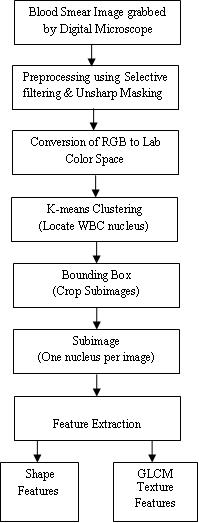
\includegraphics[scale=0.6]{schemat_Automated_Leukemia_Detection_in_Blood_Microscopic}
	\caption{Obraz pochodzi z pracy \cite{Mohapatra:2011:ALD:1947940.1947980}}
\end{figure}

Etapy zmodyfikowanego algorytmu obejmują:
\begin{itemize}
\item Wzmacnianie kontrastu (imadjust)
\item Filtr medianowy (medfilt)
\item Konwersja RGB -> Lab
\item K-mean Clustering
\item Zastosowanie regionprops i wybór mniejszego regionu 
\item Zastosowanie erozji na tym regionie 
\item Ponowne zastosowanie regionprops
\item Zaznaczenie wszystkich wykrytych za drugim razem regionów, prócz największego
\end{itemize}

\paragraph{K-mean Clustering\\}
Podobnie jak w przypadku pracy \cite{Mohapatra:2011:ALD:1947940.1947980} w przetwarzaniu obrazu zostaje wykorzystana technika K-mean Clustering. Pozwoliła ona na wydzielenie dwóch oddzielnych obszarów na obrazie. Jeden z nich powinien być tłem, a drugi zawierać potencjalne niepożądane zmiany/guzy. Ten etap zostaje wykonany za pomocą funkcji kmeans.

\paragraph{Regionprops\\}
Do wyciągnięcia informacji z obszaru wydzielonego przez K-mean Clustering zastosowana zostaje funkcja regionprops. Wyciąga ona różne informacje na temat części obrazu. W przypadku tego algorytmu jest stosowana dwa razy. Najpierw na obrazie całego obszaru, aby wyodrębnić mniejszą jego część, na której może się znajdować potencjalny guz. Potem na tym otrzymanym obszarze, uprzednio przetworzonym dodatkowo przez erozję. Dane z tego drugiego wywołania funkcji służą już jako pozycje wykrytych potencjalnych anomalii.


\subsection{API}
Funkcje:
\begin{itemize}
\item contourResults - funkcja odpowiedzialna za wyznaczenie obwiedni wokół znalezionych anomalii; przyjmuje tablicę struktur z przetworzonymi zdjęciami, zwraca tablicę struktur z wyznaczonymi konturami każdej anomalii
\item displayAll - funkcja służy do wyświetlania w jednym oknie zdjęcia źródłowego i czarno - biały efekt detekcji
\item displayAllColored - funkcja odpowiedzialna za wyświetlenie wyników; jako wejście przyjmuje tablicę struktur z oryginalnymi zdjęciami oraz tablicę struktur konturów wyznaczonych dla nich, wyświetla czerwoną obwiednię wokół anomalii dla każdego zdjęcia
\item entropyYen - funkcja wyznacza próg binaryzacji na podstawie metody Yena; jako wejście podawane jest zdjęcie w skali szarości, zwraca liczbę z przedziału 0-255
\item getAllData - funkcja służy do ładowania zdjęć z bazy ,,http://peipa.essex.ac.uk/pix/mias/all-mias.tar.gz''
\item processScans - funkcja, odpowiedzialna za przetworzenie obrazów z danego zakresu metodą I
\item processScans2 - funkcja, odpowiedzialna za przetworzenie obrazów z danego zakresu metodą II
\end{itemize}
Skrypty:
\begin{itemize}
\item przetwarzamy - główny moduł programu
\end{itemize}

\subsection{Opis interfejsu użytkownika}
Przed pierwszym uruchomieniem należy skopiować folder, zawierający pliki programu w programie Matlab na swój dysk. Aby zacząć przetwarzać zdjęcia należy otworzyć ten folder, a następnie uruchomić skrypt ,,przetwarzamy.m''. Program spyta o zakres zdjęć, które chcemy przetworzyć (indeks dolny i górny). Po podaniu prawidłowego zakresu program będzie kontynuował działanie. Wynikiem finalnym jest okno z obrazem oryginału, obrazem z zaznaczonym obszarem uzyskanym za pomocą metody I oraz obrazem przetworzonym według metody II, na którym również zostały zaznaczone potencjalne anomalie.

\bibliography{bibliografia}
\bibliographystyle{alpha}
\end{document}